\documentclass[12pt,a4paper,oneside]{book}
\usepackage[latin1]{inputenc}
\usepackage[dutch]{babel}

% Voor subfiles
\usepackage{subfiles}

% Voor todo's
\usepackage{todonotes}

% Voor wiskunde
\usepackage{amsmath}
\usepackage{amsfonts}
\usepackage{amssymb}
\usepackage{amsthm}

% Voor urls
\usepackage{hyperref}

% Een mooier bestand met wiskunde ondersteuning
\usepackage{libertine}
\usepackage[libertine]{newtxmath}

% Om het totaal aantal pagina's te tellen
\usepackage{lastpage}
\usepackage{afterpage}

% Om figuren op de juiste plaats te krijgen
\usepackage{float}

% Voor frames
\usepackage{mdframed}

% Om de marges aan te passen
\usepackage[left=2cm,right=2cm,top=2cm,bottom=2cm]{geometry}


%indices
\usepackage{makeidx}
\makeindex


\theoremstyle{plain}
\newtheorem{thm}{Theorem}[chapter] %Reset counter elk hoofdstuk
\theoremstyle{definition}
\newmdtheoremenv{de}[thm]{Definitie} % Definitie met frame
\newtheorem{ei}[thm]{Eigenschap}
\newtheorem{st}[thm]{Stelling}
\newtheorem{gev}[thm]{Gevolg}
\newtheorem{pr}[thm]{Propositie}
\newtheorem{opm}[thm]{Opmerking}
\newtheorem{vb}[thm]{Voorbeeld}
\newtheorem{tvb}[thm]{Tegenvoorbeeld}
\newtheorem{lem}[thm]{Lemma}
\newtheorem{oef}[thm]{Oefening}
\newmdtheoremenv{al}[thm]{Algoritme}

\newcommand{\deref}[1]{\footnote{Zie definitie \ref{#1} op pagina \pageref{#1}.}}
\newcommand{\stref}[1]{\footnote{Zie stelling \ref{#1} op pagina \pageref{#1}.}}
\newcommand{\eiref}[1]{\footnote{Zie eigenschap \ref{#1} op pagina \pageref{#1}.}}
\newcommand{\gevref}[1]{\footnote{Zie gevolg \ref{#1} op pagina \pageref{#1}.}}
\newcommand{\prref}[1]{\footnote{Zie propositie \ref{#1} op pagina \pageref{#1}.}}
\newcommand{\opmref}[1]{\footnote{Zie opmerking \ref{#1} op pagina \pageref{#1}.}}
\newcommand{\vbref}[1]{\footnote{Zie voorbeeld \ref{#1} op pagina \pageref{#1}.}}
\newcommand{\tvbref}[1]{\footnote{Zie tegenvoorbeeld \ref{#1} op pagina \pageref{#1}.}}
\newcommand{\lemref}[1]{\footnote{Zie lemma \ref{#1} op pagina \pageref{#1}.}}
\newcommand{\alref}[1]{\footnote{Zie algoritme \ref{#1} op pagina \pageref{#1}.}}
\newcommand{\secref}[1]{\footnote{Zie sectie \ref{#1} op pagina \pageref{#1}.}}

\newcommand{\hint}[1]{Hint: #1}

% Mooiere TODO's
\newcommand{\TODO}[1]{\todo[color=red,inline,size=\small]{TODO: #1}}
\newcommand{\extra}[1]{\todo[color=orange,inline,size=\small]{EXTRA: #1}}
\newcommand{\clarify}[1]{\todo[color=yellow,inline,size=\small]{CLARIFY: #1}}
\newcommand{\question}[1]{\todo[color=green,inline,size=\small]{QUESTION: #1}}

\newcommand{\waarom}[0]{\clarify{waarom?}}
\newcommand{\needed}[0]{\clarify{referentie?}}

\newcommand{\term}[1]{\index{#1}\textbf{#1}}
\newcommand{\zb}[0]{{\footnotesize {\it Zonder bewijs\/}}}

% Opzoeken
\newcommand{\formularium}[2]{(Formularium: #1: #2)}
\newcommand{\tabel}[2]{(Tabel #1: #2)}

% Badges
\newcommand{\examen}[0]{\bx{{\bf Examenvraag!}}\\}

% Examenvragen
\newenvironment{examenvraag}[1]
{ \par\noindent \underline{ Examenvraag #1:}}
{ \pagebreak }

\newenvironment{ex-vraag}
{\begin{mdframed}}
{\end{mdframed}}

\newenvironment{ex-antwoord}
{\par\noindent}
{}

\newcommand{\kennen}[1]{#1 (kennen)}
\newcommand{\kunnen}[1]{#1 (kunnen)}

% Voor meer plaats tussen wiskunde
\renewcommand{\arraystretch}{1.25}

% Echt een vierkantje
\renewcommand{\qedsymbol}{$\square$}

\newcommand{\1}{\mathbbmss{1}}

\begin{document}

\begin{titlepage}
\thispagestyle{empty}
\hbox{ % Horizontal box
\hspace*{0.05\textwidth} % Whitespace to the left of the title page
\rule{1pt}{\textheight}
\hspace{1pt}
\rule{2pt}{\textheight}
\hspace{2pt}
\rule{3pt}{\textheight}
\hspace{3pt}
\rule{4pt}{\textheight}
\hspace*{0.05\textwidth} % Whitespace between the vertical line and title page text
\parbox[b]{0.75\textwidth}{ % Paragraph box which restricts text to less than the width of the page

\textsc{\LARGE KU Leuven}\\[1.5cm] 

{\noindent\Huge\bfseries Kansrekenen \\[0.5\baselineskip] [B-KUL-G0W66A]}\\[2\baselineskip] % Title
{\large \textit{Notities}}\\[4\baselineskip]
{\Large \textsc{Tom Sydney Kerckhove}}\\[4\baselineskip]


\begin{large}
  \begin{tabular}{l l}
    Gestart & 8 februari 2015\\
    Gecompileerd & \today\\
  \end{tabular}
\end{large}

\vspace{0.05\textheight}

\emph{Docent:} \\
Prof. Tim \textsc{Verdonck}\\



\vspace{0.2\textheight}}}
\end{titlepage}


\tableofcontents

\subfile{voorkennis}
\subfile{combinatoriek}
\subfile{kansruimten}
\subfile{stochastische-veranderlijken}
\subfile{bivariate-verdelingen}
\subfile{benaderingen-van-verdelingen}

\subfile{voorbeelden}
\subfile{oefeningen}

\bibliographystyle{plain}
\bibliography{kansrekenen-notities}


\includepdf[pages=-]{assets/tabellen.pdf}
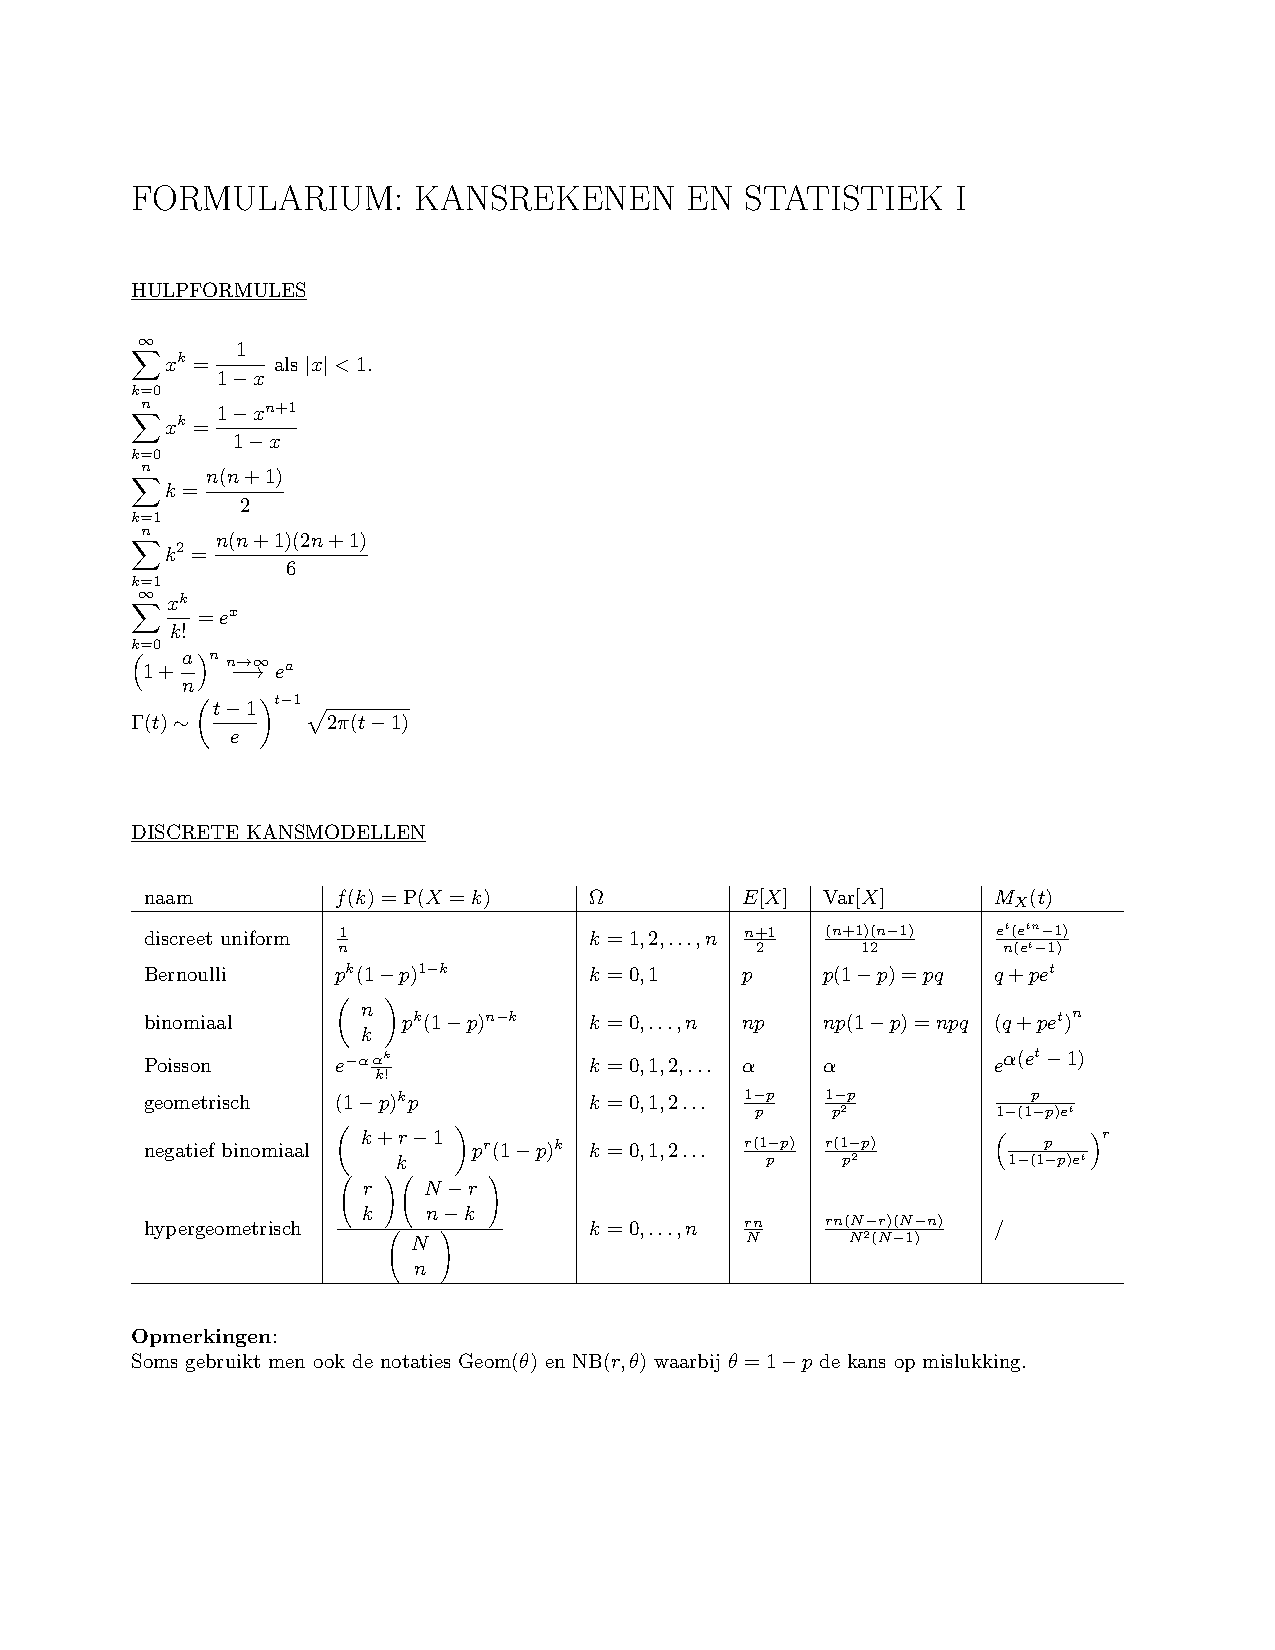
\includepdf[pages=-]{assets/formularium.pdf}

\listoftodos

\end{document}
